\documentclass[parskip=half*,fontsize=12pt,abstract]{scrartcl}
\usepackage{scrhack}
\usepackage{geometry}
\geometry{a4paper, top=2cm, left=2.5cm, right=3cm, bottom=2cm,footskip=1cm}
\usepackage{setspace}

\usepackage[utf8]{inputenc}
\usepackage[T1]{fontenc}
\usepackage{lmodern}
\usepackage[ngerman]{babel}
\usepackage[ngerman=ngerman-x-latest]{hyphsubst}
\usepackage{amsmath}
\usepackage[autostyle=true, german=quotes]{csquotes}
\PassOptionsToPackage{hyphens}{url}
\usepackage[pdfpagelabels]{hyperref}
\usepackage[nottoc,notlot,notlof]{tocbibind}
%\usepackage[htt]{hyphenat} 

\usepackage{graphicx}
\usepackage{pdfpages}
\usepackage{tikz}
\usepackage{todonotes}
\usepackage{mdframed}
\usepackage{changepage}
\usepackage{listings} %Für Code
\usepackage[german,onelanguage,boxed]{algorithm2e}%Für Pseudocode
\usepackage{enumitem}
\usepackage{mdwlist}
\usepackage{tcolorbox}
\usepackage{tabularx}
\usepackage{longtable}

\newcolumntype{L}[1]{>{\raggedright\arraybackslash}p{#1}} % linksbündig mit Breitenangabe
\newcolumntype{C}[1]{>{\centering\arraybackslash}p{#1}} % zentriert mit Breitenangabe
\newcolumntype{R}[1]{>{\raggedleft\arraybackslash}p{#1}} % rechtsbündig mit Breitenangabe

\newenvironment{heft}[1]{\begin{mdframed}\textbf{Hefteintrag: #1}\newline}{\end{mdframed}}
\newenvironment{tafel}[1]{\begin{mdframed}\textbf{Tafelanschrieb: #1}\newline}{\end{mdframed}}
\newenvironment{pseudocode}{\begin{algorithm}[H]
\SetKwFor{ForEach}{Wiederhole für alle}{}{Ende}
}{
\end{algorithm}}

\newcommand{\syso}[1]{\texttt{#1}}
\newcommand{\zitat}[1]{\enquote{\textit{#1}}}

\definecolor{light-gray}{gray}{0.95}
\newcommand{\class}[1]{\colorbox{light-gray}{\texttt{#1}}}

\begin{document}
\onehalfspacing
\pagestyle{empty}
\begin{titlepage}
{\centering
Ludwig-Maximilians-Universität München\\
Fakultät für Mathematik, Informatik und Statistik\\
Department Institut für Informatik
\vspace{1.5cm}

{\huge\bfseries	Entwicklung eines neuartigen Tower Defense Spieles}
\Large
\vspace{1.5cm}

vorgelegt von: Benjamin Knorr \\
MatrikelNr: 10967090\\[1cm]
\textbf{Ausarbeitung\\
 Praktisches Programmieren}\\[1cm]
Betreuende Dozentin: \\
Paola Maneggia

\vfill
}
Schopenhauerstraße 66, 80807 München \\
Knorr.Benjamin@campus.lmu.de\\
München, den \today
\end{titlepage}

\tableofcontents 
\newpage
\pagestyle{plain}

\section{Projektidee} % (fold)
\label{sec:projektidee}



\subsection{Bisherige Tower Defense Spiele}

Das Tower Defense Genre..... Das Grundkonzept ist dabei immer, dass der Spieler mehrere Wellen an KI-Gegnern, sogenannte \enquote{Creeps}, auf einer Karte davon abhalten muss, bestimmte Ziele zu erreichen. Dazu kann er Türme platzieren, die die Creeps töten. In den meisten Fällen handelt es sich um eher kleinere Spiele, wie Browser-, Flash- oder Mobile Games und auch die ersten bekannteren TD Spiele sind als Custom Maps im Warcraft oder StarCraft MapEditor entstanden und haben daher kein großes Entwicklerteam im Hintergrund. Der Umfang war damit für das eigene Projekt gut abschätzbar und der vorgesehenen Bearbeitungszeit angemessen. Vereinzelt wurde das Spielprinzip aber auch in größeren Produktionen, wie \todo{\dots}, aufgegriffen, was die Erweiterbarkeit des Ansatzes zeigt. Es existieren bereits einige Spielvariationen, über die im Folgenden exemplarisch ein Überblick gegeben werden soll.

\paragraph{Klassisches Spiel}
In der häufigsten (da einfachsten) Spielimplementierung bewegen sich die Creeps auf einem vordefinierten Pfad und die Türme werden entlang des Pfades frei oder auf bestimmten Knotenpunkten positioniert.Typischer Weise gibt es unterschiedliche Türme und verschiedene Creep-Arten. Zum Teil haben diese auch Spezialfähigkeiten, wie fliegende Creeps (folgen also nicht dem Pfad, sondern bewegen sich auf direkter Linie zum Ziel) bzw. Türme, die besonders gut gegen Bodeneinheiten oder gegen fliegende Einheiten sind. Häufig werden die Creeps auch in ihrer Geschwindigkeit variiert und es existieren Türme, die Creeps verlangsamen sowie Creeps die dagegen immun sind.  Diese Spiele rücken besonders das taktisch geschickte Kombinieren der verschiedenen Türme und das Aufrüsten an entscheidenden Knotenpunkten in den Fokus des Spielerlebnisses.

\missingfigure{Screenshot of normal Game}

\paragraph{Mazing Tower Defense}
Eine weitere Variante sind die \enquote{Mazing Tower Defense Spiele}, in denen die Creeps sich nicht auf einem vordefinierten Pfad bewegen, sondern der Spieler mit den Türmen eine Labyrinth artige Struktur baut, durch die die Creeps dann durchlaufen. Das erste Spiel dieser Art und daher prototypisch ist \enquote{Desktop Tower Defense} aus dem Jahr 2007 von Paul Preece, das bereits in den ersten zwei Monaten 15 Millionen Mal gespielt wurde und inzwischen durch eine Erneuerung als Facebook Anwendung noch populärer geworden. Das Spielprinzip erweitert das normale Spiel um eine strategische Planung der Kreaturenführung durch das Labyrinth um die Türme möglichst effektiv aufrüsten zu können. Die Spielelemente sind dabei weiterhin die klassischen Kreaturenarten und Turmvarianten.

\missingfigure{Screenshot of Desktop Tower Defense}

\paragraph{Andere Varianten} Es existieren noch viele weitere Varianten wie das sehr erfolgreiche Plants vs Zombies, bei dem die Creeps (=Zombies) die Türme angreifen und keine Wegfindung implementiert ist, das aber eine sehr große Vielfalt an verschiedenen Gegnern und Strategien einbringt, oder auch Multiplayer Spiele. Diese waren jedoch keine Inspirationsquelle für das eigene Projekt und werden daher nicht genauer betrachtet.

\subsection{Neuer Ansatz im eigenen Projekt}

Mazing Tower Defense erweiterte das klassische Spiel um die Herausforderung ein möglichst effektives Labyrinth zu bauen. Dabei ist jedoch die Wegsuche der Creeps optimal, wodurch zwar Labyrinthe aber keine Irrgärten entstehen. Denn Verzweigungen und Sackgassen nehmen nur unnötigen Platz weg und die Creeps werden nie in diese Bereiche hineinlaufen. Die Spielidee für dieses Projekt ist, dass die Anlage eines komplizierten Irrgartens dem Spieler einen Vorteil für das Spiel bringen soll. Um dies zu ermöglichen wurde die Prämisse aus dem Spiel genommen, dass die Kreaturen einen allwissenden Überblick über das Labyrinth haben. Stattdessen sollten sie das Labyrinth erkunden müssen. Diese Variation hatte viele Designentscheidungen zur Folge, die im Folgenden kurz vorgestellt werden.

\missingfigure{Vergleich Labyrinth in Tower Defense vs. Irrgarten}

\paragraph{State der Kreaturen} In den bisherigen Spielvarianten benötigten die Kreaturen keine eigene Repräsentation der Welt. Dagegen müssen die Creeps sich nun individuell auf Grundlage ihres bisherigen Wissens über die Welt bewegen. Ein wichtiges Spielelement ist daher die Klasse \lstinline{VisitedMap}, mit der jede Kreatur in einem zweidimensionalen Enum-Array dieses Wissen speichert. Andererseits sollen die Kreaturen auch über eine gewisse Intelligenz verfügen und nicht alle in die selbe Sackgasse laufen. Das gelingt durch simulierte Besprechungen zwischen den Kreaturen Die Karten müssen also effizient synchronisierbar sein. \todo{Link auf später}

\paragraph{Wegfindung} Die effiziente Wegfindung ist ebenfalls schwieriger: Während bei normalen TD Spielen gar keine Berechnung notwendig ist und bei Mazing TD ein A*-Algorithmus effizient den kürzesten Weg von allen Kartenpunkten zum Ziel berechnen kann, muss der Algorithmus hier noch weiter abgewandelt werden, da die Creeps nicht nur ein Ziel haben. Es muss daher für jeden Creep ein eigenes Ziel ausgewählt werden, was zum Beispiel durch wiederholte Nearest-Neighbor-Suche umgesetzt werden kann.

\paragraph{Variationsmöglichkeiten} Dadurch, dass die Kreaturen ihre eigene Wegfindung haben und Absprachen treffen, ergeben sich neue Möglichkeiten der Variation der Creeps. Beispielsweise wurden Figuren implementiert, die sich nur zufällig bewegen, andere versuchen jedes Feld der Welt zu besuchen. Weitere Möglichkeiten wären Kreaturen, die tatsächlich sehen können und damit z.B. größere Flächen direkt durchqueren, oder Kreaturen die andere dirigieren. Auch neue Turmarten, die auf diese Wegfindung Einfluss haben, sind möglich. Als Beispiel wurde dafür ein Amnesie-Turm programmiert, der die Wegsuche der abgeschossenen Creeps eine gewisse Zeit lang zu zufällig ändert.

\paragraph{Labyrinthänderungen} Die für das Genre typischen Echtzeit-Änderungen des Labyrinths sind in der Variante schwieriger an Kreaturen zu kommunizieren. Da die Creeps den Zustand ihrer erkundeten Welt speichern, sind Änderungen in bereits erkundeten Bereichen problematisch. Es gibt mehrere Möglichkeiten damit umzugehen, die in der Entwicklung abgewogen und mit User-Testings betrachtet wurden:
\begin{itemize}
	\item Kreaturen erhalten kein Update über die Welt. Bei dieser Lösung musste ein Verhalten implementiert werden, falls Creeps denken es gäbe keinen Ausweg. Typischer weise greifen eingesperrte Figuren die Türme an oder rennen darüber, was in der eigenen Variante so implementiert wurde. Das User Feedback zeigte, dass das Verhalten der Creeps insb. wegen der Kommunikation nicht nachvollziehbar ist.
	\item Kreaturen erhalten ein Update, falls sie den Bereich bereits erkundet hatten. Dies führte in User-Testings zu Strategien gegen das Spielprinzip, bei denen zwei Türme auf verschieden Seiten der Karte immer abwechselnd neu gebaut und später wieder abgerissen wurden, sodass die Kreaturen immer von einem Ende zum anderen laufen mussten.
	\item Türme können gar nicht abgerissen werden, oder nur wenn kein lebender Creep diesen erkundet hat. Dies schränkt die Möglichkeiten der Spieler zwar ein, ist aber besser verständlich und bleibt dem Spielprinzip treu.
\end{itemize}

% section projektidee (end)
\section{Entwicklungsprozess} % (fold)
\label{sec:entwicklungsprozess}

Bei dem Entwicklungsprozess wurde auf mehrere professionelle Elemente besonderen Wert gelegt. Diese sollen im Folgenden kurz erläutert werden.
\subsection{Werkzeuge} % (fold)
\label{sub:werkzeuge}
\paragraph{Versionsverwaltung} % (fold)
\label{par:versionsverwaltung}
Eine der grundlegendsten Dinge bei der Softwareentwicklung ist ein Versionskontrollsystem. In diesem Projekt wurde dafür \emph{Git} verwendet und in einem Repository auf Github (\url{https://github.com/Knorrke/MazeRunner}) veröffentlicht. Dies ermöglichte zum einen unkompliziert das Arbeiten auf mehreren Geräten. Zum anderen konnte durch das Erstellen neuer Branches seperat an Features entwickelt werden, ohne die Hauptversion während dem Entwicklungsprozess zu verändern. Über Pull Requests wurden die Features dann in den Hauptzweig gemerget.
% paragraph versionsverwaltung (end)

\paragraph{Dependency Managagement} % (fold)
\label{par:dependency_managagement}
Um nicht jedes Mal das Rad neu zu erfinden, ist es oft sinnvoll existierende Bibliotheken zu verwenden. Damit das Projekt leicht auf anderen PCs eingerichtet werden kann, sollte das Einbinden von solchen Abhängigkeiten durch ein Verwaltungssystem geschehen. Dafür wurde \emph{Maven} verwendet, das ebenfalls eine Buildautomatisierung ermöglichte.
% paragraph dependency_managagement (end)

\paragraph{Continuous Integration} % (fold)
\label{par:continuous_integration}
Mit einem Continuous Integration Service (in diesem Fall \emph{Travis CI}) konnte sichergestellt werden, dass die Tests nicht nur auf dem eigenen Gerät funktionieren, sowie dass Pull Requests vollständig funktionsfähig sind bevor sie in den Hauptzweig eingebunden werden. Des Weiteren ließ sich dadurch das Testcoverage Tool \emph{JaCoCo} integrieren (Genaueres siehe \ref{sub:testgetriebene_entwicklung}).
% paragraph continuous_integration (end)
% subsection werkzeuge (end)

\subsection{Testgetriebene Entwicklung} % (fold)
\label{sub:testgetriebene_entwicklung}

Für die Gewährleistung der Funktionalität und Absicherung für Änderungen sind Unit-Tests enorm hilfreich. Sie verkürzen die Zeit zur Fehlersuche, da Fehler direkt mit einem Knopfdruck angezeigt werden können. Außerdem geben sie dem Entwickler Sicherheit bei größeren Strukturänderungen, dass das System danach noch die Anforderungen erfüllt. Das Projekt wurde komplett testgetrieben entwickelt. Diese Methode beschreibt das Vorgehen, vor der Implementierung bereits den Test zu schreiben, also zu definieren wie der Code sich verhalten soll. Anschließend wird dieser Test so einfach wie möglich erfüllt. Dadurch wird sichergestellt, dass nur Code geschrieben wird, der auch wirklich notwendig ist. In einer dritten Phase, dem Refactoring, wird der Code anschließend nochmal bzgl Code-Qualität überarbeitet. Dabei hilft der bereits definierte Test zu überprüfen, ob die Funktionalität nach dem Refactoring immer noch gegeben ist. 

Ein Testcoverage Tool ermöglicht anschließend zu überprüfen, ob auch alle Teile des Codes durch Tests abgedeckt sind. In diesem Projekt liegt die Testabdeckung zur Zeit der Abgabe bei 98\%. Die restlichen 2\% betreffen überwiegend das Loggen von evtl. auftretenden \class{IOExceptions}, die nicht extra für Tests erzeugt wurden.

Um die Tests eines Codeteiles besser von dem Verhalten des restlichen Codes trennen zu können, wurde zudem das Mocking Framework \emph{Mockito} verwendet. Das ermöglicht es, für Klassen und Interfaces eine Art Attrappe zu erzeugen, für die dann konfiguriert werden kann, wie er auf bestimmte Methodenaufrufe mit den korrekten Argumenten reagiert. Zum Einen kann dadurch der zu testende Code besser isoliert werden, weil keine Abhängigkeiten zu anderen Klassen existieren. Es kann aber auch überprüft werden, ob die Aufrufe richtig stattgefunden haben, ob also die Interaktion mit dem Mock-Objekt so ablief, wie erwartet. Dadurch lässt sich auch die Integration in den restlichen Softwareaufbau gut testen.
\missingfigure{Beispielcode von Mockito}
% subsection testgetriebene_entwicklung (end)


\subsection{JavaFX} % (fold)
\label{sub:javafx}
Für die Umsetzung der Benutzeroberfläche wurde JavaFX verwendet, das durch die Abwandlung des Observer-Patterns auch viel Einfluss auf den Softwareentwurf hatte (siehe Kapitel \ref{sub:observer}). Das Framework ermöglichte eine modern wirkende Oberfläche durch viele vorgefertigte Komponenten und zahlreiche verfügbare Erweiterungen, wie z. B. ein Popup-Menü. Dabei wird die Komplexität von Swing für ansprechende Layouts deutlich reduziert und das meiste geschieht für den Programmierer unsichtbar im Hintergrund. Zudem existiert für JavaFX Anwendungen das Projekt \emph{javafxports}, das ermöglicht den gesamten Code ohne große Anpassungen direkt in Mobile Apps zu packen.

Für die testgetriebene Entwicklung ist die View-Programmierung eine Herausforderung. Hierfür konnte jedoch mit \emph{TestFX} (\url{https://github.com/TestFX/TestFX}) ein gutes Framework verwendet werden, das eine schnelle und anschauliche Implementierung von Unit-Tests für JavaFX ermöglicht. Dadurch konnte auch die korrekte Reaktion auf (erwartete) Userinteraktionen überprüft werden.
\missingfigure{Beispielcode von TestFX}
% subsection javafx (end)
% section entwicklungsprozess (end)
\section{Softwaredesign} % (fold)
\label{sec:softwaredesign}

Um den Code leicht erweitern zu können und Fehlern vorzubeugen, ist es wichtig, den Aufbau der Software gut zu strukturieren. Dabei gibt es einige typische Probleme, für die bereits etablierte Lösungen existieren. Diese Design Pattern helfen nicht nur dabei, den Code wartbar zu halten, sondern helfen auch in der Kommunikation mit anderen Entwicklern bei strukturellen Problemen. In diesem Kapitel soll ein Highlevel-Überblick über die Softwarestruktur und verwendete Design Muster gegeben werden.

\subsection{Model View Controller} % (fold)
\label{sub:model_view_controller}
Eines der wohl am weitesten verbreitete Entwurfsmuster ist das Model View Controller Pattern, das auch in dieser Arbeit umgesetzt wurde. Es trennt die verschiedenen Aufgaben einer Software in drei Bereiche auf: Daten und Spiellogik bilden das Modell, das in sich funktioniert und nach außen Schnittstellen bietet, die dann interne Spielprozesse auslösen. Getrennt davon ist die View, deren Aufgabe einzig darin besteht, die Daten aus dem Modell (evtl. gefiltert) dem Spieler anzuzeigen. Diese View ist mit JavaFX geschrieben, wobei die Trennung vom restlichen Code teilweise durch die Verwendung von \emph{FXML} besonders deutlich wird. Die View muss dabei Änderungen aus dem Modell mitbekommen und daraufhin entsprechend anzeigen. Die View stellt zudem Schnittstellen zur Verfügung, um auf bestimmte Useraktivitäten zu reagieren. Diese Schnittstellen verwendet der Controller. Er setzt also Listener auf Komponenten der View für verschiedene User Interaktionen wie Mausklicks, Hovering oder Tastatureingaben. Die Listener sind größtenteils als anonyme Klassen implementiert und rufen bei einer Aktion die entsprechenden Schnittstellen des Modells auf.  
% subsection model_view_controller (end)

\subsection{Observer Pattern} % (fold)
\label{sub:observer}
Im Zusammenspiel mit MVC ist das Observer Pattern eines der wichtigsten. Es ermöglicht eine lose Kopplung zwischen View und Modell, indem sich die View beim Modell als Observer registriert und das Modell bei Änderungen alle Observer benachrichtigt. Dadurch ist gewährleistet, dass das Modell nicht explizit die View kennen muss und so kann die View leichter ausgetauscht werden oder weitere Views (z.B. auch Sounds) angebunden werden, ohne in das Modell einzugreifen. In JavaFX funktioniert die Umsetzung ein wenig anders, nämlich mittels \enquote{Bindings}: Das Modell bietet Properties an, auf denen Listener registriert werden können, die aber auch direkt an Viewausgaben gebunden werden können. Beispielsweise stellt die Geldanzeige im Spiel einen formatierten String der \class{IntegerProperty money} des \class{PlayerModel} dar. Da immer das aktuelle Geld angezeigt werden soll, kann hierfür ein Binding verwendet werden, statt den Umweg über einen Listener zu nehmen.
% subsection observer (end)

\subsection{Game Loop} % (fold)
\label{sub:gameloop}
Eine Game Loop löst das Problem, die Spielzeit mit der Realzeit zu synchronisieren, statt ihren Ablauf von User-Interaktionen (wie bei klassischen EVA), abhängig zu machen oder von der Prozessorgeschwindigkeit abhängig zu sein \cite{gameloopPattern}. Die Implementierung richtet sich nach \cite{gameloopImpl, gameloopImplFX} und verwendet drei Elemente:
\begin{itemize}
	\item \textbf{Synchronisation mit der Realzeit}: Messe wie viel Realzeit seit der letzten Spielzeit Simulation vergangen ist und simuliere ungefähr diese Zeitspanne (Einschränkungen siehe die nächsten zwei Punkte).

	\item \textbf{Feste Zeitschritte}: Eine Frame Rate über 60 Bilder pro Sekunde ist nicht notwendig, daher wird versucht diese Zielrate ungefähr zu erreichen. Kürzere Zeitschritte werden also zusammengefasst, bis \(1/60\) Sekunde zusammenkommen, größere Zeitschritte werden in mehrere 1/60 Sekunden Schritte zerteilt und einzeln simuliert. Dadurch bleibt das Spiel deterministisch -- im Gegensatz zur Verwendung von variablen Zeitschritten.

	\item \textbf{Begrenzte Zeitschritte}: Ist der Prozessor zu langsam, um eine Iteration in \(1/60\,s\) auszuführen, ist bei der nächsten Iteration mehr Zeit vergangen, wodurch er mehr Zeitschritte machen muss, die wieder länger dauern, etc. Um diese Spirale zu verhindern, wird die vergangene Zeit auf eine bestimmte Länge beschränkt. Die Nachteil daran ist, dass das Spiel auf zu langsamen Prozessoren langsamer läuft.
\end{itemize}

Interpolation der Zeitschritte wurde nicht eingebaut, da diese Komplexität sich in alle Komponenten fortsetzt, die von der Game Loop synchronisiert werden sollen.

Wegen JavaFX wurde die \class{GameLoop} als Spezialisierung des \class{AnimationTimer} erstellt, der automatisch durch den JavaFX-Thread aufgerufen wird. Durch das Binding konnten die Zeitupdates der View aus der Game Loop entfernt werden, da sie bei Änderungen des Modells bereits ihre internen Werte ändern und vom JavaFX-Thread aktualisiert werden.
% subsection gameloop (end)

\subsection{Strategy Pattern} % (fold)
\label{sub:strategy_pattern}
Das Strategy Pattern wird verwendet, um den Ablauf eines Algorithmus zur Laufzeit ändern zu können. Man erstellt Objekte, die die Implementierung des Algorithmus beinhalten und verwendet dann Komposition der Objekte. Dadurch können auch viele unterschiedliche Algorithmen für die selbe Klasse implementiert werden, ohne Unterklassen zu verwenden. Dies entspricht auch dem Prinzip der Objekt Orientierung \enquote{composition over inheritance}, durch das eine lose Kopplung erreicht werden kann. Verwendet wurde dieses Pattern bei der Wegfindung der Creeps. Die Klasse \class{RandomMovement} implementiert eine völlig zufällige Bewegung und Berücksichtigt nur Wände. Diese wird von den einfachsten Kreaturenarten verwendet, die nur am Anfang auftauchen. Dagegen sucht \class{NoSightMovement} mit einer abgewandelten Dijkstra-Suche das nächste unbekannte Feld (bezieht also bereits besuchte Felder ein) und bewegt sich zu diesem hin. Dabei werden jedoch nur Felder auf besucht gesetzt, die tatsächlich abgelaufen wurden. Eine weitere mögliche Klasse, die nicht mehr implementiert wurde, ist \class{SightMovement}, die alle Felder auf besucht setzt, die von der aktuellen Position aus gesehen werden können und erst dann nach einem unbekannten Ziel sucht. Ebenso wäre eine Klasse \class{PerfectMovement} denkbar, die dem kürzesten Weg zum Ziel durch das Labyrinth verfolgt, wie es normalerweise in Tower Defense Spielen üblich ist.

\begin{figure}[htb]
	\centering
	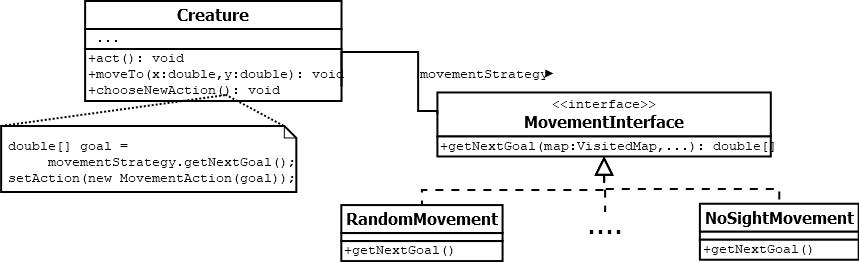
\includegraphics[width=\linewidth]{images/strategy-pattern.png}
	\caption{Strategy Pattern bei der Wegfindung}
\end{figure}

Dass diese Algorithmen zur Laufzeit ersetzt werden können, bietet die Möglichkeit für interessante Kreaturen-Interaktionen und Tower-Arten: Mit dem \class{AmnesiaTower} wurde ein Turm implementiert, der die Creeps durch seine Schüsse verwirrt. Dabei ersetzt er für eine kurze Zeit den eigentlichen Wegfindungsalgorithmus der Kreatur durch \class{RandomMovement}. Genauso könnte man Creeparten implementieren, die anderen beim Kommunizieren bessere Strategien beibringen, also z.B. \class{RandomMovement} der einfachsten Kreaturen durch \class{SightMovement} ersetzen. Ebenfalls angedacht sind Kommandeure, die -- statt selbst durch das Labyrinth zu rennen -- auf Türme klettern und von dort mit Überblick über das gesamte Labyrinth die anderen Creeps durchlotsen können, also die Bewegung durch \class{PerfectMovement} ersetzen. 

Auch Algorithmusimplementierungen, die gar nicht darauf abzielen das Labyrinth zu durchqueren, wären möglich. Beispielsweise könnten intelligentere Kreaturen an geschützten Stellen warten oder priorisiert zu anderen Kreaturen laufen, um diesen Informationen weiterzugeben. Das Projekt bietet hier wie man sieht noch einige Erweiterungen, die bisher noch nicht implementiert werden konnten. Die Grundfunktionalität, um solche Features umzusetzen, sind allerdings mit dem Strategy Pattern gelegt und am Beispiel des Amnesie-Turms auch verwendet.
% subsection strategy_pattern (end)


\subsection{Static Factory Method} % (fold)
\label{sub:static_factory_method}
Gemeint ist hier nicht das Factory Method Pattern, sondern eine statische Methode zur Erzeugung eines Objektes einer Klasse. Im Gegensatz zum Konstruktor hat die Static Factory Method die Möglichkeit auch Objekte von Unterklassen zu erzeugen oder ein bereits erzeugtes Objekt zurückzugeben. In diesem Sinne verwendet z.B. auch das Singleton Pattern eine Static Factory Methode. Dieses Vorgehen wurde sowohl für Türme verwendet, bei denen der Aufruf konkrete Objekte der Unterklassen erzeugt, sowie für die Kreaturen. Bei letzteren ist die Erzeugung etwas umfangreicher und mit verschiedenen Parametern möglich und wurde zur Übersichtlichkeit daher in eine eigene Klasse \class{CreatureFactory} ausgelagert. Diese Factory kann dann z. B. anhand des Types und des Zeitfortschritts die Leben und den Wert der Creeps, sowie deren Bewegungsstrategie bestimmen und entsprechend den Konstruktor der \class{Creature} aufrufen. Dadurch wird die Erzeugung der Figuren besser gekapselt.

% subsection static_factory_method (end)
% section softwaredesign (end)
\section{Überblick der wichtigsten Programmteile} % (fold)
\label{sec:überblick_der_wichtigsten_programmteile}

Im Folgenden wird auf die wichtigsten Teile des Programms nochmal genauer eingegangen und einzelne relevante Algorithmen und Datenstrukturen beschrieben und reflektiert.

\subsection{Model} % (fold)
\label{sub:model}
Das Model teilt sich in drei Hauptkomponenten auf: Die Spielerverwaltung (Leben und Geld) im Paket \class{model.player}, die Levelverwaltung (Zeitlicher Ablauf der Wellen) im Paket \class{model.level} und die Spielwelt an sich im Paket \class{model.maze} mit Kreaturen und Türmen. Das \class{PlayerModelInterface} und die implementierende Klasse \class{Player} sind sehr einfach (eigentlich nur Resourcen erhöhen / verringern) und werden daher nicht genauer betrachtet. Auf die anderen beiden Teile wird dagegen im Folgenden noch genauer eingegangen, wobei die Spielwelt aufgrund der Komplexität noch weiter unterteilt wird. Grundlegend für beide sind Aktionen, die zunächst kurz erklärt werden.

\subsubsection{Akteure und Aktionen} % (fold)
\label{ssub:aktionen}
Alle Objekte, die im Rahmen der Spielzeit agieren, implementieren das \class{ActorInterface} -- ein Funktionales Interface, das nur eine Methode \class{void act(double dt)} beinhaltet. Alle Akteure können beliebig auf das Fortschreiten der GameZeit reagieren. Häufig ist die Entscheidung, was als nächstes getan wird, jedoch nicht bei jedem Tick zu treffen, sondern kann in eine gewisse Spanne andaurnde Aktionen untergliedert werden. Die Klasse \class{Action} bietet eine abstrakte Implementierung eines Akteurs, der solange eine bestimmte Aktion durchführt, bis eine Abbruchbedingung erfüllt ist. Konkrete Implementierungen davon sind \class{CountdownAction}, die als Abbruchbedingung das Ablaufen einer Zeitspanne hat, sowie \class{MoveAction}, die als Abbruchbedingung das Erreichen eines gewissen Punktes oder beweglichen Objektes hat. Diese Klassen bieten die Grundlage für alle wiederholenden Aktionen.
% subsubsection aktionen (end)
\subsubsection{Das Paket \texttt{level}} % (fold)
\label{ssub:level}

Die Aufgabe des Level Pakets ist wie gesagt die zeitliche Steuerung der Creep-Wellen. Sie bietet nach außen für die View ein Binding, wie viel Prozent des Spiels schon vergangen sind. Nach einem gewissen Countdown erstellt sie -- entsprechend der Konfiguration des aktuellen Levels -- eine Liste von Kreaturen in der \class{CreatureFactory} und beauftragt das \class{MazeModelInterface} diese in das Spiel einzufügen. Anschließend wird der Countdown neu gestartet.
% subsubsection level (end)

\begin{figure}[htb]
  \centering
  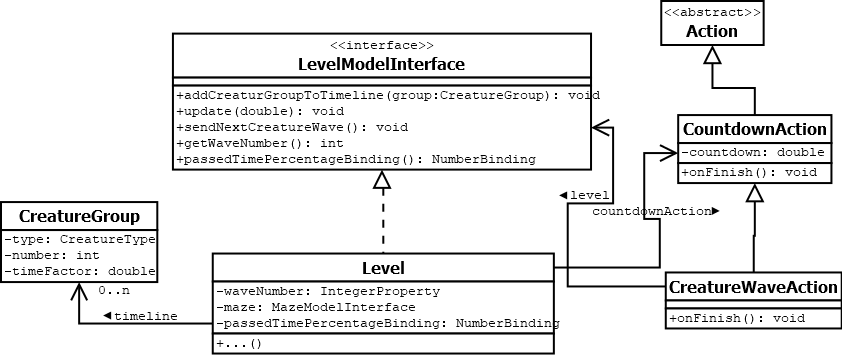
\includegraphics[width=\linewidth]{images/level-package.png}
  \caption{Das Klassendiagramm des \texttt{level} Packages (vereinfachte Darstellung).}
\end{figure}

\subsubsection{Das Paket \texttt{maze} -- Kreaturen} % (fold)
\label{ssub:maze_kreaturen}
Vieles zu den Kreaturen wurde bereits in den vorherigen Kapiteln (insb \ref{sub:strategy_pattern}) erklärt. Im Folgenden wird sich daher auf bisher noch nicht erwähnte Strukturen fokusiert.

Es gibt verschiedene Kreaturenarten, die in einem Enum \class{CreatureType} spezifiziert sind. Dieses Enum enthält auch die Default-Werte der Typen für die Leben, Geschwindigkeit, Wert und Bewegungsalgorithmus. Ausgehend von diesen Default-Werten werden die Creeps in der \class{CreatureFactory} mit einem bestimmten Zeitfaktor abgewandelt (Kreaturen werden mit der Zeit stärker, geben aber auch etwas mehr Geld).

\begin{lstlisting}[caption={Enum der Kreaturen Arten mit Konfiguration der default Werte (gekürzt).}, captionpos=b]
public enum CreatureType {
  DUMB(3, 10, 1, new RandomMovement()),
  NORMAL(1, 10, 1, new NoSightMovement()),
  TOUGH(0.8, 30, 3, new NoSightMovement());
  //... Attribute mit Gettern
  private CreatureType(double defaultVelocity, int defaultLifes, int defaultValue, MovementInterface defaultMovement) {
   //... Zuweisung
  }
}
\end{lstlisting}

Die Kreaturen sind Akteure und werden daher von der GameLoop aktualisiert. Sie besitzen eine aktuelle \class{Action}, die z.B. eine \class{MoveAction} zu einem bestimmten Ziel ist. Ist dieses Ziel erreicht, sucht die Kreatur mit dem gesetzten Bewegungsalgorithmus das nächste Ziel und erstellt dafür eine neue MoveAction. Zusätzlich wird bei jeder Positionsänderung überprüft, ob Kreaturen in der Reichweite sind, die andere Informationen über die Spielwelt haben (\class{VisitedMap}). Falls das der Fall ist, wird die Bewegungsaktion durch eine \class{CountdownAction} vorübergehend unterbrechen, um sich mit der anderen Kreatur zu unterhalten. Danach wird die Bewegung fortgesetzt.

\begin{figure}[htb]
  \centering
  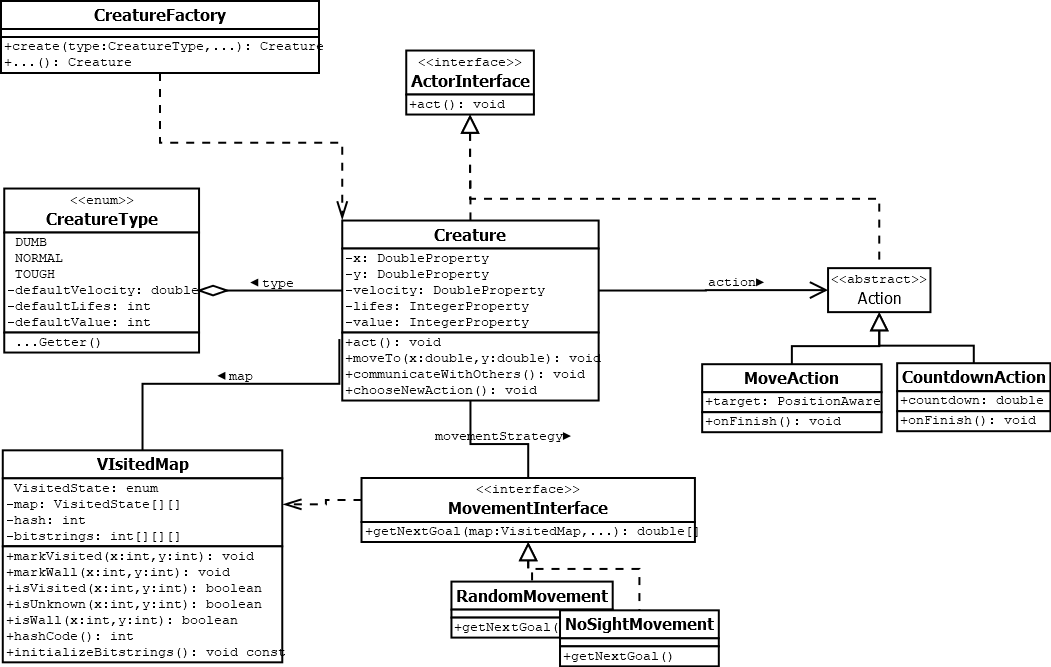
\includegraphics[width=\linewidth]{images/creature-classdiagram.png}
  \caption{Das Klassendiagramm der Creature Klassen (vereinfachte Darstellung). Anm.: Die Darstellung der \class{MovementInterface} Implementierungen veranschaulicht das Strategy-Pattern.}
\end{figure}
\paragraph{VisitedMap} % (fold)
\label{par:visitedmap}
Wie bereits in Kapitel~\ref{sub:neuer_ansatz_im_eigenen_projekt} erwähnt, ist die VisitedMap zentraler Bestandteil der scheinbaren Intelligenz der Kreaturen. Da diese sehr oft verglichen wird, war hier eine effiziente Implementierung notwendig. Die Speicherkomplexität der Map liegt in \(O (c\cdot n \cdot m)\), wobei \(c\) die Anzahl der Creeps, und \(n\times m\) die Abmessung der Spielwelt ist (im aktuellen Spiel \(10\times20\)). Sind jedoch alle \(c\) Kreaturen nah zusammen, versucht jede Kreatur mit jeder anderen zu kommunizieren, also \(c\cdot (c-1)\) und jeder Vergleich der Arrays benötigt \(O(n\cdot m)\) Schritte \(\Rightarrow O(c^2\cdot n\cdot m)\). Eine Optimierung gelingt dadurch, dass für die Arrays ein Hash-Wert erstellt wird und für den Vergleich herangezogen wird. Nur wenn die Hash-Werte unterschiedlich sind, wird über das gesamte zweidimensionale Array iteriert und die Informationen zusammengefügt. Dadurch muss in dem gleichen Fall nur eine Kreatur mit allen anderen den Zustand synchronisieren -- alle anderen Vergleiche sind unabhängig von der Spielfeldgröße \(\Rightarrow O(c\cdot n \cdot m + (c-1)\cdot(c-1)\cdot1) = O(c \cdot n \cdot m + c^2) \). Da sich die Figuren in der Regel eine längere Zeit in der Gruppe bewegen, unterscheidet sich der State auch seltener, wodurch der Vorteil des Hashwertes noch deutlich wird. Nicht beachtet wurde dabei bisher die Komplexität zur Berechnung des Hash-Wertes. Zunächst wurde die Methode \class{Arrays.deepHashCode(Object[] a)} zur Berechnung verwendet, die allerdings in Benchmarks immer noch eine hohe Auslastung anzeigte. Stattdessen wurde anschließend das Zobrist Hashing \cite{zobrist1970new} verwendet (genaueres siehe nächster Abschnitt). Das ermöglichte, den Hash-Wert bei Änderungen direkt mit einer einfachen Bit-Operation anzupassen, statt ihn mit dem gesamten Array neu zu berechnen. Dies führte zu einem vernachlässigbaren Aufwand zur Hashberechnung und der Vergleich war effizient genug, dass dies kein Problem mehr darstellte. Die tatsächlich gemessenen Laufzeitergebnisse sind in Abbildung~\ref{fig:benchmark} dargestellt.
\begin{figure}[htb]
	\centering
	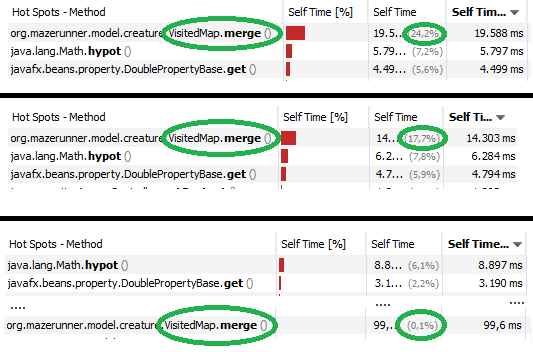
\includegraphics[width=0.8\linewidth]{images/benchmark.png}
	\caption{Laufzeitanalyse der drei Implementierungen der Merge-Methode mit JavaVisualVM. Die Daten zeigen einen Ausschnitt der rechenintensivsten Methoden gemessen zur Laufzeit mit 600 Kreaturen und dem gleichen Labyrinth Setup. Die erste Tabelle zeigt die Laufzeit ohne Hashing, die zweite mit \lstinline{Arrays.deepHashCode}, die dritte die letztliche Programmierung mit Zobrist Hashing.}
	\label{fig:benchmark}
\end{figure}

\subparagraph{Ablauf des Zobrist Hashing} % (fold)
 \label{subp:ablauf_des_zobrist_hashing}
 Beim Zobrist Hashing werden einmalig für jedes Feld in jedem möglichen Zustand ein Bitmuster (in Form eines zufälligen Integers) erzeugt.
\begin{lstlisting}
public class VisitedMap {
  private static int[][][] bitStrings;
  public enum VisitedState { UNKNOWN, VISITED, WALL }

  private void initializeBitStrings(int maxX, int maxY) {
    if (bitStrings == null) {
      bitStrings = new int[maxX][maxY][VisitedState.values().length];
      for (int x = 0; x < maxX; x++) {
        for (int y = 0; y < maxY; y++) {
          for (int j = 0; j < VisitedState.values().length; j++) {
            bitStrings[x][y][j] = new Random().nextInt();
          }
        }
      }
    }
  }
  /* ... */
}
\end{lstlisting}
Der Hash wird dann pro \class{VisitedMap} Objekt (also pro Kreatur) einmal gebildet, indem ausgehend von dem Hash 0 für jedes Feld der VisitedMap das entsprechende Bitmuster mit \emph{XOR} mit dem Hash verknüpft wird. 
\begin{lstlisting}
  private VisitedState[][] map;
  private int hash = 0;

  public VisitedMap(int maxX, int maxY) {
    initializeBitStrings(maxX, maxY);
    map = new VisitedState[maxX][maxY];
    for (int x = 0; x < map.length; x++) {
      for (int y = 0; y < map[x].length; y++) {
        map[x][y] = VisitedState.UNKNOWN;
        hash ^= bitStrings[x][y][VisitedState.UNKNOWN.ordinal()];
      }
    }
  }
\end{lstlisting}
Änderungen können dann einfach vorgenommen werden, indem zuerst mit \emph{XOR} der alte Wert aus dem Hash rausgenommen wird (denn \emph{XOR} ist seine eigene Umkehrfunktion) und der neue Wert mit \emph{XOR} hinzugefügt wird.
\begin{lstlisting}
private void setNewStateOnPosition(int x, int y, VisitedState newState) {
  VisitedState old = map[x][y];
  hash ^= bitStrings[x][y][old.ordinal()] ^ bitStrings[x][y][newState.ordinal()];
  map[x][y] = newState;
}
\end{lstlisting}
 % subparagraph ablauf_des_zobrist_hashing (end)
% paragraph visitedmap (end)

\paragraph{Wegsuche} Von der konkreten Algorithmik interessant ist bei der Pfadfindung nur die Klasse \class{NoSightMovement}. Das Vorgehen wurde schon in Kapitel~\ref{sub:strategy_pattern} kurz beschrieben. Die Aufgabe des Algorithmus ist es, aus der aktuellen \class{VisitedMap} und der aktuellen Position ein nächstes Ziel zu bestimmen. In Betracht gezogen wurden dafür alle noch unbekannten Felder, also ist das naheste, unbekannte Feld gesucht. Die einfachste Implementierung war, eine Breitensuche wie im Dijkstra-Algorithmus zu beginnen und bei dem ersten unbekannten Feld abzubrechen. Da diese Berechnung nicht in jedem Tick ausgeführt wird, sondern nur wenn eine neue Aktion berechnet wird (bei den normalen Kreaturen also einmal pro Sekunde), ist die Performanz hiervon auch kein Problem gewesen. Tatsächlich ist eine Verbesserung hier gar nicht so leicht: Überlegt war zum Beispiel, ob der Algorithmus beschleunigt werden kann, indem für das gesamte Labyrinth einmalig z.B. mit dem Floyd-Warshall-Algorithmus von allen Punkten aus der kürzeste Weg zu allen anderen Punkten berechnet wird. Statt für jede Aktion den Dijkstra-Algorithmus erneut auszuführen, müsste so nur bei einer Änderung des Labyrinths neuberechnet werden. Das Problem ist allerdings, dass den Kreaturen diese Tabelle nicht so viel nützt, weil sie ihr Ziel nicht kennen, sondern anhand der bereits bekannten Felder ein weiteres suchen wollen. Ebenso ist die Suche mit Dijkstra für diese Aufgabe sehr gut geeignet. Eine algorithmische Verbesserung in diesem Bereich schien also bisher nicht notwendig und konnte von mir auch noch nicht gefunden werden.

\paragraph{Datenstruktur der Kreaturen} Ein Bereich, der im Rahmen des Projektes noch nicht optimiert wurde, ist die Datenstruktur der Kreaturen. Diese sind in einer \class{ObservableList} gespeichert, was der View erlaubt einen \class{ChangeListener} darauf zu registrieren. Die Datenstruktur wurde verwendet, da die Implementierung am einfachsten war, jedoch ist sie ein Engpass für die Berechnungen im Model und aktuell der langsamste Teil im Projekt. Grund dafür ist, dass besonders häufig Bereichsanfragen auf die Kreaturen gestellt werden, beispielsweise wenn ein Tower zum Schießen bereit ist, oder wenn Kreaturen miteinander Kommunizieren wollen. Dementsprechend wäre wahrscheinlich eine Speicherung in einem k-d Baum oder R-Baum effizienter. Das Problem daran ist, dass die Kreaturen sich sehr viel bewegen und somit entweder häufig die aufwändigen Update-Operationen auf den Bäumen ausgeführt werden müssen, oder die Bäume zu jedem Tick mit Bulkload neu erstellt werden müssen. Das stellt einen hohen Anspruch an die Effizienz der Bäume dar.
% subsubsection maze_kreaturen (end)

\subsubsection{Das Paket \texttt{maze}: Türme} % (fold)
\label{ssub:maze_türme}

Grundbausteine zum bilden des Labyrinths sind zunächst Mauern. Diese haben sehr geringe kosten und blockieren die Creeps. Jede Mauer hat eine \class{ObjectProperty} vom generischen Typ \class{AbstractTower}, kann also durch Polymorphie ein beliebiges Objekt der Unterklassen von \class{AbstractTower} besitzen. Diese Unterklassen sind die konkreten Türme, die eigene Upgrades definieren und eine Methode \class{void shoot()} implementieren müssen.

Um ständige \class{null} Überprüfungen zu vermeiden, wurde auch eine Unterklasse \class{NoTower} implementiert, die keinerlei Aktivität übernimmt. Die weiteren Turmarten sind:
\begin{itemize}
  \item \class{NormalTower}: Ein Turm, der nur einmal pro Sekunde schießt, dafür aber relativ stark ist und der billigste Turm ist. Upgrades erhöhen vor allem die Stärke und Reichweite des Turms. Dieser Turm ist die Orientierung für die Stärke der anderen Türme.
  \item \class{FastTower}: Schießt schneller, aber schwächer und kostet etwas mehr. Upgrades sind dafür billiger und verstärken vor allem die Geschwindigkeit und Stärke.
  \item \class{SlowdownTower}: Macht keinen Schaden, sondern verlangsamt die getroffene Kreatur. Schießt selbst langsamer und kostet etwas mehr. Upgrades erhöhen die Geschwindigkeit und verstärken den Slowdown-Effekt.
  \item \class{AmnesiaTower}: Macht keinen Schaden, sondern \enquote{verwirrt} die getroffene Kreatur, indem eine Zeit lang die Wegfindung der Kreatur durch eine zufällige Wegwahl ersetzt wird. Der Turm versucht beim schießen Kreaturen zu finden, die er bisher noch nicht getroffen hat und kann so eine größere Menge an vorbeilaufenden Kreaturen treffen. Es ist der teuerste Turm, jedoch existieren keine Upgrades.
\end{itemize}

Der normale Turm ist auch die Orientierung für Game Balancing Überlegungen wie \zitat{Wie oft muss ein Turm eine normale Kreatur treffen?}, und \zitat{Wie viele Schüsse kann ein Turm auf eine vorbeilaufende Kreatur abgeben?}, nach denen sich die Leben der Kreaturen richten. Die Werte aller anderen Türme werden ebenfalls an den Daten des normalen Turms orientiert festgelegt. Eine automatisierte Anpassung basierend auf Nutzerdaten wurde nicht implementiert, wäre aber grundsätzlich möglich und eine interessante Erweiterung. 

Die Implementierung der Türme verwendet eine \class{CountdownAction}, die das Schießen nach dem entsprechenden Intervall triggert. Da wird zunächst mit einer Bereichsanfragen auf die Kreaturen ein Ziel ausgewählt. Anschließend wird eine Kugel erzeugt, die sich wiederum mit einer \class{MoveAction} zunächst zum Ziel bewegen muss, bevor sie ihre Wirkung entfaltet. Vor allem Letzteres ist wichtig, um den Effekt der Kugel bis zum tatsächlichen Treffen verzögern zu können und nicht direkt in der Schießen-Methode auszuführen. Dadurch ist der Ablauf für den User besser sichtbar und nachvollziehbar.

\begin{figure}[htb]
  \centering
  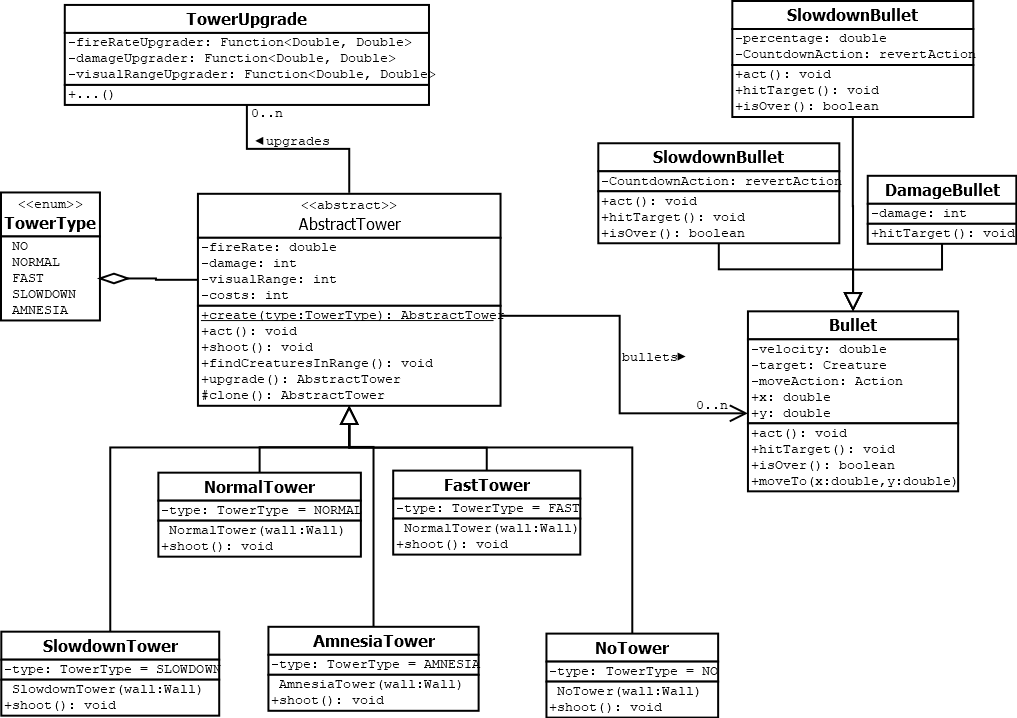
\includegraphics[width=\linewidth]{images/tower-class-diagramm.png}
  \caption{Das Klassendiagramm der Tower Klassen (vereinfachte Darstellung).}
\end{figure}


\paragraph{Upgrades}
Die Upgrades werden definiert über drei Implementierungen eines Funktionalen Interfaces, das die Schussgeschwindigkeit, den Schaden bzw. den Sichtradius anpasst. Um die \class{ObjectProperty} zu nutzen, wird nicht der aktuelle Turm verändert, sondern ein Klon erzeugt, dessen Werte angepasst und der anschließend an den Aufrufer zurückgegeben wird. 
\begin{figure}[htb]
\begin{lstlisting}
public class Wall implements ActorInterface {
  /* ... */
  public void upgradeTower() {
    setTower(getTower().upgrade());
  }
}

public abstract class AbstractTower implements ActorInterface, Cloneable {
  /* ... */ 
  public AbstractTower upgrade() {
    if (upgrades.size() > getLevel()) {
      TowerUpgrade upgrade = upgrades.get(getLevel());
      try {
        AbstractTower clone = (AbstractTower) this.clone();
        clone.fireRate = upgrade.getFireRateUpgrader().apply(getFireRate());
        clone.damage = upgrade.getDamageUpgrader().apply(getDamage());
        clone.visualRange = upgrade.getVisualRangeUpgrader().apply(getVisualRange());
        clone.costs = this.costs + upgrade.getCosts();
        clone.level = level +1;
        return clone;
      } catch (CloneNotSupportedException e) {
        LOG.log(Level.SEVERE,"couldn't clone tower", e);
      }
    }
    
    return this; //if something went wrong
  }
}
\end{lstlisting}
\end{figure}

\paragraph{Datenstruktur der Mauern} Die Datenstruktur im \class{Maze}, die die Mauern hält, ist wie bei den Kreaturen eine \class{ObservableList}. Dadurch kann die View wieder einen Listener auf die Änderungen registrieren. Da die Kreaturen oft anfragen müssen, ob auf einem Feld eine Mauer den Weg blockiert, wurde zusätzlich noch ein zweidimensionales Boolean-Array gespeichert, das allerdings nur intern verwendet wird. Der zusätzliche Speicheraufwand ist zu vernachlässigen, da nur ein einzelnes Maze existiert und somit nur ein Boolean-Array in der Größe des Spielfeldes gespeichert wird. Die Anfragezeit, ob ein Feld belegt ist, konnte dagegen dadurch auf konstante Zeit \(O(1)\) im Gegensatz zu linearer Zeit \(O(w)\) (\(w\) Anzahl der \class{Wall} Objekte) reduziert werden. 

% subsubsection maze_türme (end)
\subsubsection{Die Klasse \texttt{Game}}
Das Interface \class{GameModelInterface} und die implementierende Klasse \class{Game} ist der Einstiegspunkt im Model, der das Player-, Level- und Maze-System initialisiert und miteinander verbindet. Zusätzlich verwaltet es einen \class{GameState}, der beschreibt ob das Spiel noch in der BauPhase vor dem Start ist, gerade läuft, oder bereits beendet (gewonnen / verloren) ist.
% subsection model (end)

\subsection{View und Controller} % (fold)
\label{sub:view}

Das Grundlayout der View wurde in \emph{FXML} erstellt und besteht aus den folgenden Bereichen: Links Die Level Timeline mit den Kreaturen Wellen, daneben ein weiterer unterteilter Bereich mit den Spielerinformationen (oben), der Labyrinthfläche (Mitte) und den Kontrollbuttons (unten).

\begin{figure}[htb]
  \centering
  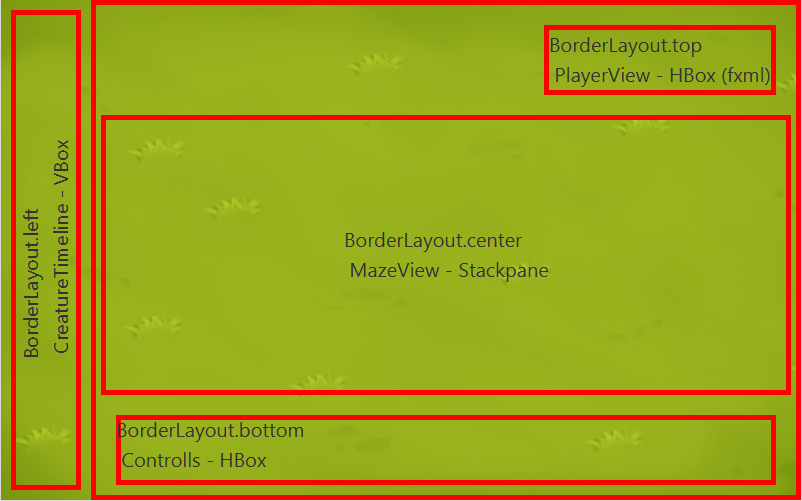
\includegraphics[width=\linewidth]{images/layout.png}
  \caption{Grundaufbau der Oberfläche, wie in fxml spezifiziert. Die Aufteilung gelang mit zwei geschachtelten \class{BorderLayout}s.}
\end{figure}

\subsubsection{CreatureTimeline} % (fold)
\label{ssub:creaturetimeline}
Die CreatureTimeline hat einen interessanten Aspekt, nämlich das scrollen mit der Spielzeit. Dafür verwendet sie das \class{passedTimePercentageBinding} aus dem LevelModelInterface und bindet an die \class{translateYProperty} aus der VBox, die die Kreaturen Gruppen enthält. Beim Klicken auf eine Kreatur der Timeline wird ein Popup mit den entsprechenden Informationen über die Kreaturen der Welle erzeugt
\begin{figure}[htb]
  \centering
  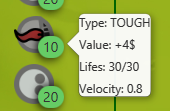
\includegraphics[width=3cm]{images/timeline.png}
  \caption{Popup mit Informationen über kommende Kreaturen.}
\end{figure}


% subsubsection creaturetimeline (end)

\subsubsection{PlayerView} % (fold)
\label{ssub:playerview}
Die PlayerView ist ebenfalls in fxml geschrieben und bindet die \class{lifesProperty} und die \class{moneyProperty} (als Geld-Text formatiert) an die Labels. 
\begin{lstlisting}
public void initModel(PlayerModelInterface player) {
  this.player = player;
  money.textProperty().bind(Util.moneyString(this.player.moneyProperty()));
  lifes.textProperty().bind(Bindings.max(0, this.player.lifesProperty()).asString());
}
\end{lstlisting}
% subsubsection playerview (end)

\subsubsection{Controls} % (fold)
\label{ssub:controls}
Die Controls sind direkt in der \texttt{GameView.fxml} enthalten, da sie keinerlei View-Aufgaben haben. Drücken des Play/Pause-Buttons ruft eine Methode auf dem GameController auf, der die GameLoop startet bzw. stoppt. Ebenso rufen die Bauen- und Info Buttons Methoden auf, die den Modus entsprechend wechseln. Im Bauen Modus werden alle Aktionen von den Controllern als Bau-aktionen interpretiert (Klick in Labyrinthfläche baut Mauer), im Informationsmodus werden keine Bauaktivitäten durchgeführt sondern wenn möglich weitere Informationen angezeigt (Klick auf Turm zeigt Informationen statt Buttons zum Abreisen).
\begin{figure}[htb]
  \centering
  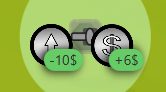
\includegraphics[width=3cm]{images/klick-bauen.png}\hspace{1cm}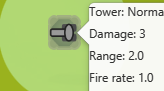
\includegraphics[width=3cm]{images/klick-informationen.png}
  \caption{Klick auf Turm im Bauen Modus (links) und Informationsmodus (rechts)}
\end{figure}
% subsubsection controls (end)

\subsubsection{MazeView} % (fold)
\label{ssub:mazeview}
Die MazeView enthält eine \class{Pane} für die Kreaturen zur beliebigen Positionierung und eine \class{StackPane} für die Türme. Dies ist leider nicht optimal, da dann entweder die KreaturenEbene unter der Turmebene oder andersrum liegen muss. Dadurch wird entweder die Lebensanzeigen und Sprechblasen der Kreaturen (in Kreaturenebene) von Türmen verdeckt werden, oder die Kugeln der Türme (in Turmebene) unter den Kreaturen durch fliegen. Hier wäre eine Neustrukturierung gut.

Von der Implementierung her arbeiten die beiden Ebenen recht ähnlich: Sie haben einen Listener auf der Liste der Creeps bzw. Mauern im Model und erstellen bzw. entfernen dementsprechend \class{CreatureView} bzw. \class{WallView}, die sie als Kinder verwalten.

\begin{lstlisting}
public class CreaturesView extends Pane implements Bindable<MazeModelInterface> {
    ListChangeListener<Creature> listener =
      (c) -> {
        while (c.next()) {
          if (c.wasAdded()) {
            createCreatures(c.getAddedSubList());
          } else if (c.wasRemoved()) {
            removeCreatures(c.getRemoved());
          }
        }
      };

  @Override
  public void bind(MazeModelInterface maze) {
    /* ... */
    creatures.addListener(listener);
  }
  /* ... */
}
\end{lstlisting}
Wird eine Kreatur entfernt, erstellt die Kreaturenebene ein Label für das gewonnene Geld, zeigt es kurz an und entfernt es dann wieder.

\paragraph{CreatureView}
Die Klasse \class{CreatureView}, die für die Anzeige einer einzelnen Kreatur zuständig ist, hat folgende interessante Aspekte:
\begin{itemize}
  \item Ein Listener auf den Leben der Kreatur zeigt einen Fortschrittsbalken an, sobald die Kreatur Schaden nimmt. 
  \item Ein Listener auf der Position wird verwendet um aus der Änderung die aktuelle Drehung der Kreatur zu berechnen. 
  \item Ein Listener auf der Aktion der Kreatur zeigt eine Sprechblase an, sobald die Kreatur eine \class{TalkAction} anfängt.
\end{itemize}

\paragraph{TowerView}
Die \class{WallView} ist für die Anzeige einer Mauer zuständig und verwendet intern nochmal eine \class{TowerView} für die Anzeige des Turms und der Kugeln. Der Code ist sehr einfach, das einzige spannende ist das Menü zum Turmbau und -upgrade, wenn man eine Mauer anklickt. Dafür wurde das \class{CirclePopupMenu} aus der Bibliothek \emph{jfxtras} verwendet, das die Elemente gleichmäßig in einem Kreis anordnet und auf- und zuklappen animiert.
\begin{figure}[htb]
  \centering
  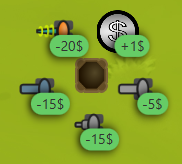
\includegraphics[width=4cm]{images/klick-turm.png}
  \caption{Popup-Menü mit der externen Klasse \class{CirclePopupMenu} zum Bauen von Türmen.}
\end{figure}
% subsubsection mazeview (end)
% subsection view (end)
\subsection{Weitere Klassen} % (fold)
\label{sub:weitere_klassen}
Für das Projekt wurden noch einzelne Hilfsklassen programmiert, die größtenteils statisch verwendet werden. Beispielsweise bietet \class{Util} Methoden zur Berechnung der Distanz zwischen zwei Punkten, oder zur Berechnung des Winkels eines Vektors. Besonders elegant ist der \class{ImageLoader}. Dieser bietet einen statischen Zugriff auf die Bilder und verhindert so, dass diese mehrmals geladen werden oder die Logik zum Laden von Bildern sich im Code verteilt. Die Bilder werden dort versucht zu laden, wobei nicht existierende Bilder durch einen Platzhalter ersetzt werden. Das ermöglichte die Grafiken unabhängig von den Features zu entwickeln.
\begin{lstlisting}
public class ImageLoader {  
  private static final String basePath = "images/";
  private static Image placeholder = loadImage("placeholder.png");
  private static Image normalCreature;
  /* ... */

  public static void loadGameImages() {
    normalCreature = loadImage("creatures/normal.png");    /* ... */
  }

  private static Image loadImage(String src) {
    InputStream resourceStream =
        ImageLoader.class.getClassLoader().getResourceAsStream(basePath + src);
    if (resourceStream != null) {
      return new Image(resourceStream);
    } else if (placeholder != null) {
      return placeholder;
    }

    LOG.severe("Image loading unsuccessfull!");
    throw new Error("Failed loading Image " + src);
  }
}
\end{lstlisting}
% subsection weitere_klassen (end)
% section überblick_der_wichtigsten_programmteile (end)

\newpage
\thispagestyle{empty}
{\Large \textbf{Eidesstattliche Versicherung}}

\textbf{Erklärung zur Hausarbeit gemäß §29 (Abs.6) LPO I}

Hiermit erkläre ich, dass die vorliegende Hausarbeit von mir selbstständig verfasst wurde und dass keine anderen als die angegebenen Hilfsmittel benutzt wurden. Die Stellen der Arbeit, die anderen Werken dem Wortlaut oder Sinn nach entnommen sind, sind in jedem einzelnen Fall unter Angabe der Quelle als Entlehnung kenntlich gemacht. 

Diese Erklärung erstreckt sich auch auf etwa in der Arbeit enthaltene Zeichnungen, Kartenskizzen und bildliche Darstellungen. 

\vspace{2cm}

\begin{tabular}{lcl}
    \hspace{5cm} & \hspace{2cm} & \hspace{7cm} \\
    \dotfill & & \dotfill \\
    Ort, Datum & & Name
\end{tabular}

\end{document}
